%%==================================================
%% chapter03.tex for SJTU Bachelor Thesis
%% version: 0.5.2
%% Encoding: UTF-8
%%==================================================

% \bibliographystyle{sjtu2} %[此处用于每章都生产参考文献]

\chapter{Performance Evaluation}
\label{chap:evaluation}

In this section, we will use several experiments to show the performance of our centralized and distributed load balancing schemes. The traffic in this system will be changed once in a while, and then we will use the load balacing schemes and check whether the reference index of the network is minimized in corresponding conditions. And in the evaluation part, we will also compare the number of migrated switches in different conditions.

\vspace{-5pt}
\section{Experiment Environment}

As the predecessors having done in their experiment, we deploy 10,000 switches and 100 controllers in a $100m \times 100m$ square. There is a switch in every $1 \times 1 \text{ m}^2$ square, and thus each switch is $1m$ away from switches in its neighborhood. Meanwhile, the controllers are evenly distributed in this system. That is to say, each controller is in the center of a $10 \times 10 \text{ m}^2$ square. In this network, each controller is allowed to communicate with other controllers that are within a circle with radius to be $40m$. And each controller can monitor switches that are within a circle that has a radius to be $30m$. And the weight of each switch follows Pareto distribution with the parameter $\alpha=3$. Meanwhile, in LCM-LBMC and SPCM-LBMC, we set the capacity of each controller to be 300 times a random number that obeys Pareto ditribution. And the switch priority to each controller is decided by the distance between the switch and the controller. In our experiment, we define the switch priorty (value) of switch $s_j$ to controller $c_i$ to be $v_{ij}$. $v_{ij}=3$ if the distance $d(i, j)$ between $c_i$ and $s_j$ is smaller than or equal to $10m$ : $d(i, j) \le 10m$; $v_{ij}=2$ if the distance $10m < d(i, j) \le 20m$; $v_{ij}=1$ if the distance $20m < d(i, j) \le 30m$; and $v_{ij}=2$ if the distance $d(i, j) > 30m$. And we set the parameters $\alpha = 0.8, \beta = 1.2, \gamma = 1.5$. In some related works, some scholars have proved that with these parameters, the performance will reach a maximum. Thus, we omit the discussion of influence on these parameters, and only focus on the difference between different schemes.

However, the performance of these schemes are also relative to the number of controllers in the network, or we can say that it is relative to the ratio of controllers to switches. For 10,000 switches in our system, the more controllers we have, the more balanced this system will become. This is very intuitive. If we deploy many controllers in the network, they will share the switches, and thus make the system balanced. Meanwhile, in this condition, each switch will also have more reachable controllers, and can have more choices in the migrating process. Otherwise, many switches may only be monitored by a certain controller, and thus forbids the migration. Since the influence of the number of controllers is very clear and have already been proved in other documents, we also skip the discussion of that.

Then using the configuration above, we compare the performance between the naive centralized scheme and the distributed scheme.

\vspace{-5pt}
\section{Centralized Scheme VS Distributed Scheme}

\begin{figure}[!htbp]
\begin{minipage}[t]{0.45\textwidth}
    \centering
    \includegraphics[width=\linewidth]{chap5/central.eps}
    \caption{Performance of Centralized Scheme}\label{central}
  \end{minipage}\hspace{0.3cm}
  \begin{minipage}[t]{0.45\textwidth}
    \centering
    \includegraphics[width=\linewidth]{chap5/distribute.eps}
  \caption{Performance of Distributed Scheme}\label{distribute}
  \end{minipage}\hspace{0.3cm}
\end{figure}

From Figure ~\ref{central} and Figure ~\ref{distribute}, we can notice that, our LBMC schemes are effective. The weight of each switch obeys the Pareto Distribution with its parameter $\alpha=3$, and changes at different time slots. Then for both the NCM-LBMC scheme and the DM-LBMC scheme, the standard deviation decreases after the migration is done. This is because these two methods manages to move switches from overloaded controllers to idle controllers. And we can see that the performance of the naive centralized version is a little better than the distributed version. This is because the centralized controllers can get the information of the whole network, and make the best choices in the migrating process. Each switch may have a lot of destinations, and it is also possible to move a switch from controller $c_a$ to a controller $c_b$ that is very far from $c_a$. However, in the distributed version, the controllers can only get local information, and move switches to nearby controllers. This limits the scalibality of this load balancing scheme, and in this way, we make local-optimal choices instead of global-optimal choices.
\begin{figure}[!htbp]
\begin{minipage}[t]{0.45\textwidth}
    \centering
    \includegraphics[width=\linewidth]{chap5/migswitch.eps}
    \caption{The Comparison of Migrated Switches}\label{migswitch}
  \end{minipage}\hspace{0.3cm}
  \begin{minipage}[t]{0.45\textwidth}
    \centering
    \includegraphics[width=\linewidth]{chap5/fixdynamic.eps}
    \caption{Migrated Switches of DM-LBMC}\label{fixdynamic}
  \end{minipage}\hspace{0.3cm}
\end{figure}

In Figure ~\ref{migswitch}, we notice that the number of migrated switches in the centralized scheme is larger than the number in the distributed scheme. This is also because the centralized version have a global view. Every time the load in the network changes, a switch can be moved to any of its reachable controllers. But in the distributed version, a switch can only be migrated to a controller that is the neighbor of the current one. And for local hot spots, this will prohibit the migrating phase. In this part, we compare the migrating switch number of NCM-LBMC and DM-LBMC in the condition that the whole weight in the network is changing, and we can see that the migrated switches at different time slot is nearly the same. And if the weight in the system is fixed, the centralized version still holds this feature since it has a global perspective, but the distributed version no more holds it. In Figure ~\ref{fixdynamic}, the number of migrated switches remains stable in conditions with dynamic total weight. If controller $c1$ is overloaded, it will send some switches to its nearby controllers. But if in the next round, the switches that monitored by those controllers gain higher traffic load and make the nearby controllers overloaded, then the switches may be sent back to controller $c1$. And if the total weight of the system is fixed, the number of migrated switches with decreases rapidly, and then holds stable. This is because DM-LBMC only migrates locally, and as the system becomes more balanced, the scheme will only need to move a few switches to make some micro adjustments. 

\vspace{-5pt}
\section{Different Centralized Schemes}

We then examine the performance of different kinds of centralized schemes. We modified the naive centralized load balancing scheme, and raise another two schemes: NCM-LBMC and SPCM-LBMC. These two schemes take the problem of capacity limits and system value into consideration.

\begin{figure}[!htbp]
\begin{minipage}[t]{0.45\textwidth}
    \centering
    \includegraphics[width=\linewidth]{chap5/weightgraph.eps}
    \caption{Standard Deviation of limited CM-LBMC}\label{weightgraph}
  \end{minipage}\hspace{0.3cm}
  \begin{minipage}[t]{0.45\textwidth}
    \centering
    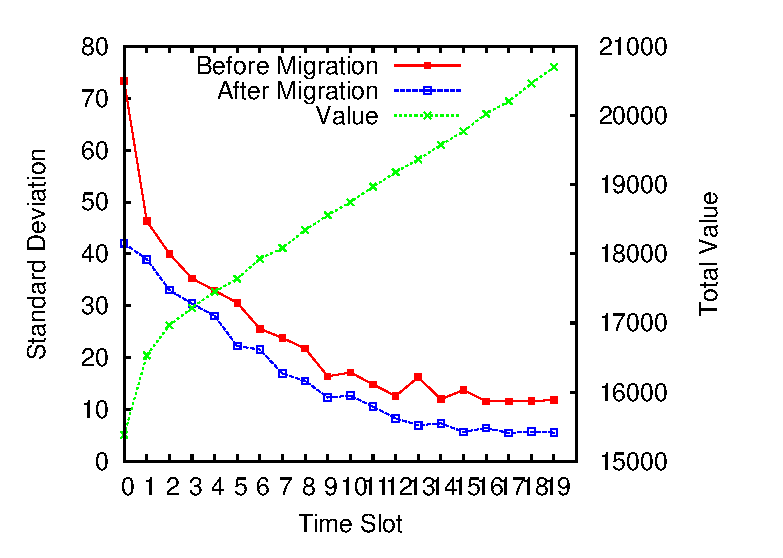
\includegraphics[width=\linewidth]{chap5/valuegraph.eps}
    \caption{Standard Deviation of Switch-Priority-based CM-LBMC}\label{valuegraph}
  \end{minipage}\hspace{0.3cm}
\end{figure}

Figure ~\ref{weightgraph} and Figure ~\ref{valuegraph} show the performance of these two modified algorithms. In limited CM-LBMC, the maximum performance of each controller also follows Pareto distribution with $\alpha=3$, and we amplify it with a constant to make sure the total traffic load not exceed the capacity of all controllers. In CM-LBMC with switch priority, we allocate a value to each mapping of a switch and a controller, which is inversely proportional to their distance. Fig. \ref{weightgraph} shows the standard deviation of our limited CM-LBMC at different time slots. We can see that the standard deviation is decreasing, but is still obviously higher than that in naive CM-LBMC. This is because in limited CM-LBMC, each controller has a different upper bound, this will influence the migration. For example, if some switches can only be monitored by a certain controller, and that controller is overloaded, then this will cause a high standard deviation since we cannot remove the switches to other controllers. It is similar in CM-LBMC with switch priority, which is shown in Figure \ref{valuegraph}. Meanwhile, in Figure \ref{valuegraph}, we show that the total value of the whole network is increasing, and the standard deviation is decreasing. And the standard deviation we get when it becomes stable is also acceptable. Thus, our schemes are effective and also practical.
